\documentclass[landscape]{article}

\title{Idea project LMECA2660}
\author{Vincent Degrooff}


\usepackage{amsmath}
\usepackage{graphicx}
\usepackage{subfigure}
\usepackage{tikz}
\usetikzlibrary{calc,patterns,decorations.pathmorphing,decorations.markings, decorations.text}
\usetikzlibrary{shapes.multipart, angles, calc, quotes}
% \usepackage{showframe}% added to show that the figure is being centered
\usepackage{geometry}
\usepackage{xcolor}
\usepackage{physics}
\geometry{left=15mm, right=15mm,top=15mm, bottom=15mm}

\begin{document}

\maketitle


\begin{figure}[!h]
    \centering
    \subfigure {
        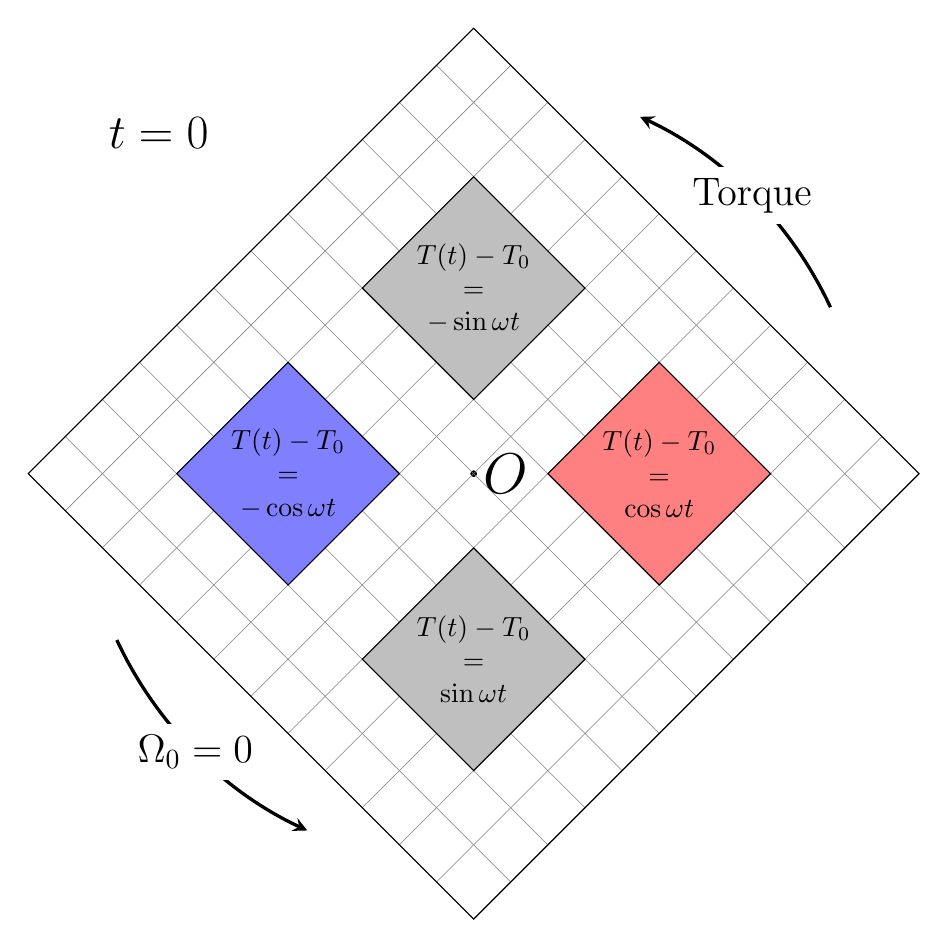
\begin{tikzpicture}[
            every text node part/.style={
                align=center
            },
            my angle/.style = {
                draw, ->, >=stealth, very thick,
                angle radius = #1,
                angle eccentricity=1.,
                anchor=center,
            },
            every pic quotes/.style = {
                inner sep=4pt,
                fill=white
            }
            ]
                        
            \pgfmathsetmacro{\theta}{45}
            \pgfmathsetmacro{\L}{4.}
            \pgfmathsetmacro{\li}{1*\L/6}
            \pgfmathsetmacro{\lii}{2*\L/3}
            \pgfmathsetmacro{\ngrid}{12}

            \coordinate (O) at (0, 0);
            \coordinate (A) at (\theta - 20:1.25*\L);
            \coordinate (B) at (\theta + 20:1.25*\L);
            \coordinate (C) at (180 + \theta - 20:1.25*\L);
            \coordinate (D) at (180 + \theta + 20:1.25*\L);

            \draw (-\L, \L) node[anchor=south]{\LARGE $t=0$};

            \filldraw[black] (0,0) circle (1pt) node[anchor=west]{\huge $O$};
            \pic [my angle=1.25*\L cm, "{\Large Torque}"]     {angle = A--O--B};
            \pic [my angle=1.25*\L cm, "{\Large $\Omega_0=0$}"]     {angle = C--O--D};

            \foreach \i in {0,...,\ngrid} {
                \draw [very thin,gray,rotate around={\theta:(0.,0.)}] (-\L, {\L * (-1. + 2*\i / \ngrid)}) -- (\L, {\L * (-1. + 2*\i / \ngrid)});
                \draw [very thin,gray,rotate around={\theta:(0.,0.)}] ({\L * (-1. + 2*\i / \ngrid)}, -\L) -- ({\L * (-1. + 2*\i / \ngrid)}, \L);
                }


            \draw[rotate around={\theta:(0.,0.)}] (-\L, -\L) rectangle (+\L, +\L);

            \foreach \c/\sx/\sy in {red/1/-1, gray/1./1., blue/-1/+1, gray/-1/-1} {
                \draw[rotate around={\theta:(0.,0.)}, fill=\c!50, fill opacity=1.] (\sx*\li, \sy*\li) rectangle (\sx*\lii, \sy*\lii);
            }

            \foreach \angle/\label in {45/$-\sin{\omega t}$, 135/$-\cos{\omega t}$, 225/$\sin{\omega t}$, 315/$\cos{\omega t}$} {
                \node at ({\theta+\angle}:{sqrt(2)*(\li+\lii)/2.}) {$T(t)-T_0$ \\ $=$ \\ \label};
            }

        \end{tikzpicture}
    }
    \hspace{1cm}
    \subfigure {
        \centering
        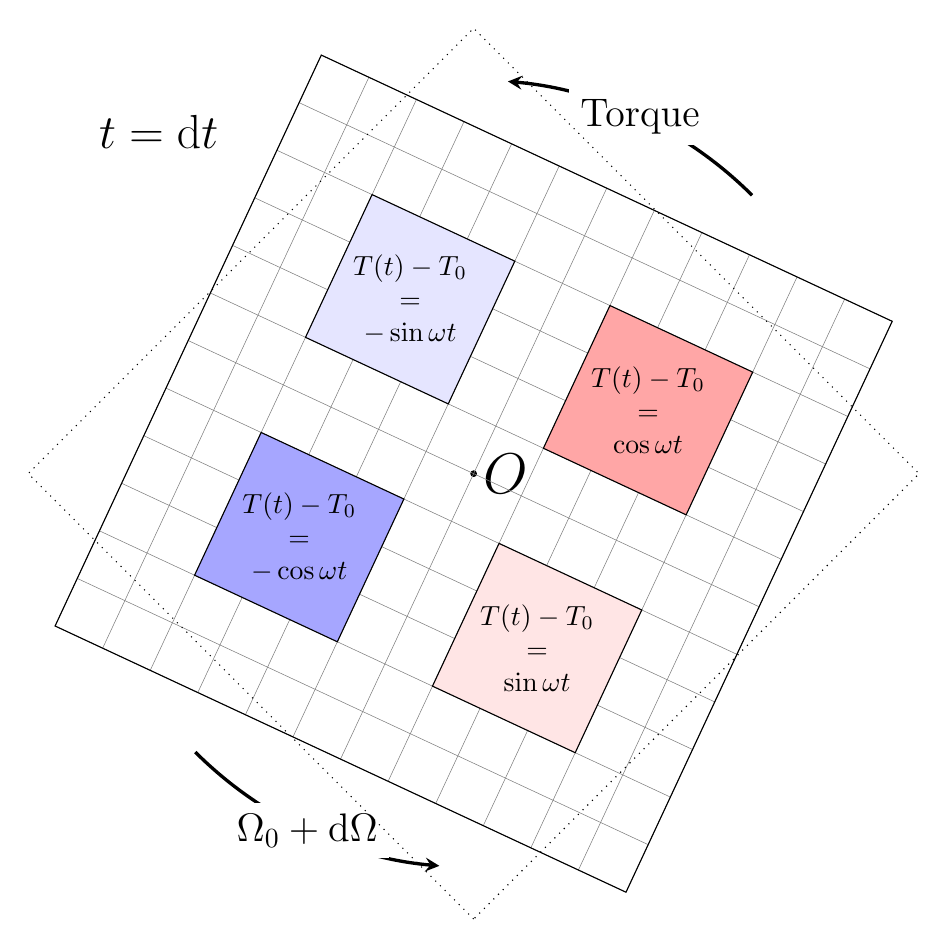
\begin{tikzpicture}[
            every text node part/.style={
                align=center
            },
            my angle/.style = {
                draw, ->, >=stealth, very thick,
                angle radius = #1,
                angle eccentricity=1.,
                anchor=center,
            },
            every pic quotes/.style = {
                inner sep=4pt,
                fill=white
            }
            ]

            \pgfmathsetmacro{\thetazero}{45}
            \pgfmathsetmacro{\theta}{65}
            \pgfmathsetmacro{\L}{4.}
            \pgfmathsetmacro{\li}{1*\L/6}
            \pgfmathsetmacro{\lii}{2*\L/3}
            \pgfmathsetmacro{\ngrid}{12}

            \coordinate (O) at (0, 0);
            \coordinate (A) at (\theta - 20:1.25*\L);
            \coordinate (B) at (\theta + 20:1.25*\L);
            \coordinate (C) at (180 + \theta - 20:1.25*\L);
            \coordinate (D) at (180 + \theta + 20:1.25*\L);

            \draw (-\L, \L) node[anchor=south]{\LARGE $t=\dd t$};

            \filldraw[black] (0,0) circle (1pt) node[anchor=west]{\huge $O$};
            \pic [my angle=1.25*\L cm, "{\Large Torque}"]     {angle = A--O--B};
            \pic [my angle=1.25*\L cm, "{\Large $\Omega_0 + \dd \Omega$}"]     {angle = C--O--D};

            \foreach \i in {0,...,\ngrid} {
                \draw [very thin,gray,rotate around={\theta:(0.,0.)}] (-\L, {\L * (-1. + 2*\i / \ngrid)}) -- (\L, {\L * (-1. + 2*\i / \ngrid)});
                \draw [very thin,gray,rotate around={\theta:(0.,0.)}] ({\L * (-1. + 2*\i / \ngrid)}, -\L) -- ({\L * (-1. + 2*\i / \ngrid)}, \L);
                }


            \draw[rotate around={\theta:(0.,0.)}] (-\L, -\L) rectangle (+\L, +\L);
            \draw[rotate around={\thetazero:(0.,0.)}, dotted] (-\L, -\L) rectangle (+\L, +\L);


            \foreach \c/\sx/\sy in {red!35/1/-1, blue!10/1./1., blue!35/-1/+1, red!10/-1/-1} {
                \draw[rotate around={\theta:(0.,0.)}, fill=\c, fill opacity=1.] (\sx*\li, \sy*\li) rectangle (\sx*\lii, \sy*\lii);
            }

            \foreach \angle/\label in {45/$-\sin{\omega t}$, 135/$-\cos{\omega t}$, 225/$\sin{\omega t}$, 315/$\cos{\omega t}$} {
                \node at ({\theta+\angle}:{sqrt(2)*(\li+\lii)/2.}) {$T(t)-T_0$ \\ $=$ \\ \label};
            }

        \end{tikzpicture}
    }
\end{figure}

\newpage

\end{document}


% \draw [
%     ->,thick,
%     postaction={
%         decorate,
%         decoration={
%             % text effects along path,text={\ {\LARGE $\Omega$}\ }, 
%             % text align=center,
%             % text effects/.cd, 
%             % text along path, 
%             % every character/.style={fill=white, yshift=-0.5ex}
%         }
%     }
% ] (-20:7) arc [start angle=-20, end angle=20, radius=7];
